\vspace{3mm}
\noindent\rqi
\vspace{3mm}

\noindent \textbf{Motivation:} As shown in previous work \cite{Potdar2014ICSME, Maldonado2015MTD}, \SATD comments can be found in the source code. However, there is not an optimal way to identify these technical debt comments yet. The methods proposed so far heavily relies on manual examination, and there are too little evidence on how well these approaches perform and how applicable they are. Answering this question is important to help us understand the opportunities and limitations of NLP techniques in identifying \SATD comments. 

\vspace{1mm}
\noindent \textbf{Approach:} As described in Section \ref{sec:approach}, we manually classify comments from ten open source projects into one of the following types of \SATD: design debt, defect debt, implementation debt, documentation debt and test debt. However, as shown in our previous work \cite{Maldonado2015MTD}, the most frequent \SATD comments are classified as design debt, implementation debt or defect debt respectively. Therefore, in our case study we focuses our attention in these three \SATD types. 

We design our case study to test how well the a maximum entropy classifier can perform when trained with our dataset. In order to do that, we first prepare the training data set. The training dataset is composed by two different columns, one is the classification and the other one is the source code comment. Then, we select all comments that were classified as not containing \SATD and the comments classified as the specific type of \SATD  that we want to predict. these comments from 9 out of 10 projects that we analyzed. Second, for the test dataset, we use the comments in the one project that was out of the training dataset and run the analysis.  

For example, if we want to classify the \SATD comments in Apache Ant project we create a training dataset using all comments from the other nine projects, namely Apache Jmeter, ArgoUML, Columba, EMF, Hibernate, JEdit, JFreeChart, JRuby and SQuirrel. Then, we use the comments of Apache Ant project to create the test dataset. 

\vspace{1mm}
\noindent \textbf{Results:} Following this approach we executed the classifier for all projects, collecting results for three different types of \SATD: design debt, implementation debt and defect debt. Tables \ref{tbl:classifier_results_design}, \ref{tbl:classifier_results_implementation} and \ref{tbl:classifier_results_defect} presents precision, recall, F1 measure, random precision, random recall and random F1 measure for each project. Taking JRuby as an example while classifying design debt in Table \ref{tbl:classifier_results_design}, we find that the classifier reached a precision of 82\% and recall of 76\% resulting in a F1 measure of 79\%. For the same project, the calculated random values for precision, recall and F1 measure are 7\%, 50\% and 13\% respectively. Comparing both F1 measures, the result obtained with the classifier is over than 6 times higher than the random one.

Regarding the results for design debt in Table \ref{tbl:classifier_results_design}, ArgoUml \SATD comments were classified with precision of 76.9\% and recall of 87.9\%, and was the higher F1 measure (i.e., 81.9\%) within our selected projects. On the contrary, EMF was classified with a precision of 52.1\%, recall of 32.1\% resulting in a F1 measure of 39.7\%. The average F1 measure considering  all projects is of 59.75\%, whereas the random F1 measure is of 8.61\%. 

For requirement debt results shown in Table \ref{tbl:classifier_results_implementation} we find that the F1 measure of the classification ranges from 11.8\% to 93.5\% for EMF and Columba. Although 11.8\% is not a very hight value the random F1 measure for EMF is less than 0\%. In average the F1 measure of all projects is of 52.28\%, and the random F1 measure is of 3.2\%. 

Lastly, for the defect debt classification results shown in Table \ref{tbl:classifier_results_defect} we achieved a F1 measure average of 25.32\% while the random F1 measure is of 1.6\%/. 
Although the F1 measure average still higher than the random F1 measure average, defect debt classification has the lowest performance. We argue that the low number of \SATD comments used in the training dataset plays a major role in this result. 

For all the types above, the random values are particularly low due to the fact that the number of comments that does not represent any kind of \SATD is much higher than the ones which represent. The number of \SATD comments are presented in Table \ref{tbl:td_distribution}. We show in this table the exact number of \SATD comments found in each project separated by the specific technical debt type: design debt, requirement debt, defect debt. Documentation debt and test debt are shown under the column `Other' as they number of occurrences were not as frequent as of the other types. 

\begin{table}[!hbt]
    \begin{center}
        \caption{Improvement over the random F1 measure for design}
        \label{tbl:improvement_f1measure_design}
        \begin{tabular}{l| c c c }
        \toprule
        \textbf{Project} & \textbf{F1} & \thead{Rnd\\F1} & \textbf{Improvement}\\
        \midrule
         Apache Ant      &  0.471      &  0.045          & 10x\\
         Apache Jmeter   &  0.704      &  0.075          & 9x\\
         ArgoUML         &  0.819      &  0.151          & 5x\\
         Columba         &  0.586      &  0.038          & 15x\\
         EMF             &  0.397      &  0.035          & 11x\\
         Hibernate       &  0.692      &  0.214          & 3x\\
         JEdit           &  0.465      &  0.037          & 12x\\
         JFreeChart      &  0.503      &  0.080          & 6x\\
         JRuby           &  0.795      &  0.131          & 6x\\
         SQuirrel        &  0.543      &  0.055          & 9x\\
        \bottomrule
        \end{tabular}
    \end{center}    
\end{table}

\begin{table}[!hbt]
    \begin{center}
        \caption{Improvement over the random F1 measure for requirements}
        \label{tbl:improvement_f1measure_requirement}
        \begin{tabular}{l| c c c }
        \toprule
        \textbf{Project} & \textbf{F1} & \thead{Rnd\\F1} & \textbf{Improvement}\\
        \midrule
         Apache Ant      & 0.462       &  0.008          & 57x\\
         Apache Jmeter   & 0.393       &  0.005          & 78x\\
         ArgoUML         & 0.741       &  0.125          & 5x \\
         Columba         & 0.935       &   0.04          & 23x\\
         EMF             & 0.118       &  0.007          & 16x\\
         Hibernate       & 0.650       &  0.042          & 15x\\
         JEdit           & 0.100       &  0.003          & 33x\\
         JFreeChart      & 0.513       &  0.011          & 46x\\
         JRuby           & 0.463       &  0.045          & 10x\\
         SQuirrel        & 0.853       &   0.04          & 21x\\
        \bottomrule
        \end{tabular}
    \end{center}    
\end{table}


\conclusionbox{We find that NLP techniques, such as maximum entropy classifiers, can be used effectively to find \SATD comments. We achieved an average F1 measure of \todo{} for design debt, an average of \todo{} while classifying requirement debt, and for defect debt our average was of \todo{}. For all three types that we classify using our dataset we perform better than the random F1 measure average, moreover our classified F1 measure is \todo{x} times better than the random F1 measure.}

\vspace{3mm}
\noindent\rqii
\vspace{3mm}

\noindent \textbf{Motivation:} After asserting the efficiency of NPL classifiers predicting \SATD we want to better understand which are the comment patterns that developers use when writing \SATD comments. Answering this question will provide insightful information that can guide future research direction and broaden our understanding on \SATD.     

\vspace{1mm}
\noindent \textbf{Approach:} As mentioned before, we use the Stanford Classifier to predict \SATD comments, and the first part of the prediction process is to generate the features that will be used to classify the comments. Features, in our case, are fragments of data that possesses a class (i.e., design debt, requirement debt or without technical debt) and a weight. These features are extracted from the comments in the training dataset, and then applied to the test dataset where they are combined to reach a vote. That is, every feature that is satisfied by the comment being classified (i.e., matched) will be used to predict the class for the comment. The vote is given to the class that has more weight, therefore positive weight features that matches the comment being classified will result in a higher weight, and the class that has the higher weight will be assumed as the predicted class.

% maybe explain more details of how the weight is given to each feature

For example, given three different features: `hack' with a weight of 5.3 , `dirty' with weigh of 3.2 both for design debt and `ignore' meaning that the comment is not a technical debt with a weight of 4.1. When classifying the following comment ``this is a dirty hack and should not be ignored'', all features would have been matched, and the vote decision would be like this: design debt weight = 8.5 (i.e., feature 1 plus feature 2) and without classification weight = 4.1 resulting in a comment classified as  design debt.

\vspace{1mm}
\noindent \textbf{Results:} Table \ref{tbl:top_ten_features} shows the top 10 features identifying \SATD in the ten studied projects ordered by weight. The first column we list the features with higher weights classifying  

\begin{table}[!hbt]
    \begin{center}
        \caption{Top ten features for Self-Admitted Technical Debt}
        \label{tbl:top_ten_features}
        \begin{tabular}{l| l c | l c }
        \toprule
        \textbf{Order} & \thead{Design\\TD} & \textbf{Weight} & \thead{Requirement\\TD}  & \textbf{Weight}\\
        \midrule
         1  & hack        &  4.9536 &  TODO:           &  4.9423 \\
         2  & workaround  &  4.8585 &  FIXME:          &  4.2058 \\
         3  & yuck!       &  4.7122 &  needed          &  4.1327 \\
         4  & kludge      &  3.0526 &  implementation  &  3.5116 \\
         5  & stupidity   &  4.6330 &  ends?           &  2.8646 \\
         6  & needed?     &  4.2578 &  Apparently      &  2.7069 \\
         7  & Unused?     &  4.2550 &  XXX             &  2.6626 \\
         8  & columns??   &  4.5500 &  configurable    &  2.5866 \\
         9  & FIXME:      &  3.8658 &  Auto-generated  &  2.5255 \\
         10 & wtf?        &  3.7930 &  Empty           &  2.3390 \\
        \bottomrule
        \end{tabular}
    \end{center}    
\end{table}

It is possible that the same feature is used to classify design debt and requirement debt. However, the weight of this feature can be different accordingly with the type being classified. As we can see in Table \ref{tbl:top_ten_features}, `FIXME:' appears in both columns although it has a higher weight when classifying requirement debt than design debt. 

In spite of the fact that features with higher weights will have more impact during the classification the final vote is given based on the combined weight of all matching features. In average the number of features to classify design debt was of 6,196 whereas for requirement debt was of 2,889.

\conclusionbox{We find that the most common comment patterns for self-admitted design debt are: `hack', `workaround', `yuck!', `kludge', `stupidity', `needed?', `unused?', `columns??', `FIXME:' and `wtf?'. Whereas, for self-admitted requirement debt, the patterns are: `TODO:', `FIXME:', `needed', `implementation', `ends?', `apparently', `XXX', `configurable', `Auto-generated' and `empty'.}

\vspace{3mm}
\noindent\rqiii
\vspace{3mm}

\noindent \textbf{Motivation:} Answering this research question will allow us to better estimate effort for future research in the area. More specifically, it will be beneficial to 1) make this kind of analysis more efficient, so manual classification of comments, that is time consuming and difficult by nature, can be kept to a minimum. 2) Helping researchers interested in applying the same technique to analyze \SATD in domains not covered in our study, another programming languages than Java, or even comments written in languages other than English. 

\vspace{1mm}
\noindent \textbf{Approach:} To be able to answer this question we executed the classification process several times with an increasing training dataset while collecting the results to analyze the changes between each iteration. 

We first select a project that will be used to create the test dataset and we keep it separated from the other nine projects. Second, we take the comments of one of the nine remainder projects to create the training dataset. Third, we run the classification process and collect the results. Fourth, we incrementally add the comments of a second project to the training dataset and repeat the classification process collecting the results. We cycle trough this steps until we had added all nine projects comments to the training dataset. 

To be throughout in this analysis, we apply this approach for each one of our ten studied projects classifying design and requirement \SATD comments. We also experimented with the order that the comments were added to the training dataset. We ranked the projects that contained more \SATD of the specific type being classified so that they can be added first to training dataset. Then, we repeat the experiment adding first the projects which has less \SATD of the specific type being classified.       

\vspace{1mm}
\noindent \textbf{Results:} While classifying design \SATD comments we find that there is significant improvement in the F1 measure during the first 3 iterations. After that, the classification will keep improving in a more stead pace. Figure \ref{fig:design_jfreechart_result} and Figure \ref{fig:design_jruby_result} shows the evolution of the F1 measure over the iterations for JFreeChart and JRuby. Each iteration of the classification is represented by a triangle in the figure, and the square stands for the random F1 measure. 

JFreeChart has F1 measure of 0.237 during the first iteration, 0.477 in the third iteration and 0.503 in the ninth iteration which was the highest F1 measure achieved. The improvement in the F1 measure between the first and third iteration is greater than the improvement between the third and ninth iteration. In the third iteration the classifier was trained with 59\% of the comments that where used in the ninth iteration. A reduction of 41\% of the necessary training data to achieve almost the same result in terms of F1 measure. 

Similarly, JRuby has a F1 measure value of 0.748 in the third iteration and 0.795 in the ninth iteration which is the maximum F1 measure achieved for the project. The F1 measure achieved in the third iteration represents 94\% of the maximum F1 measure achieved in the ninth iteration, and this percentage was reached using 1,472 comments whereas the maximum F1 measure used 2,360 comments in the training dataset. Therefore, for JRuby we could achieve 94\% of the maximum result using only 62\% of the comments.


\begin{figure}[thb!]
  \centering
  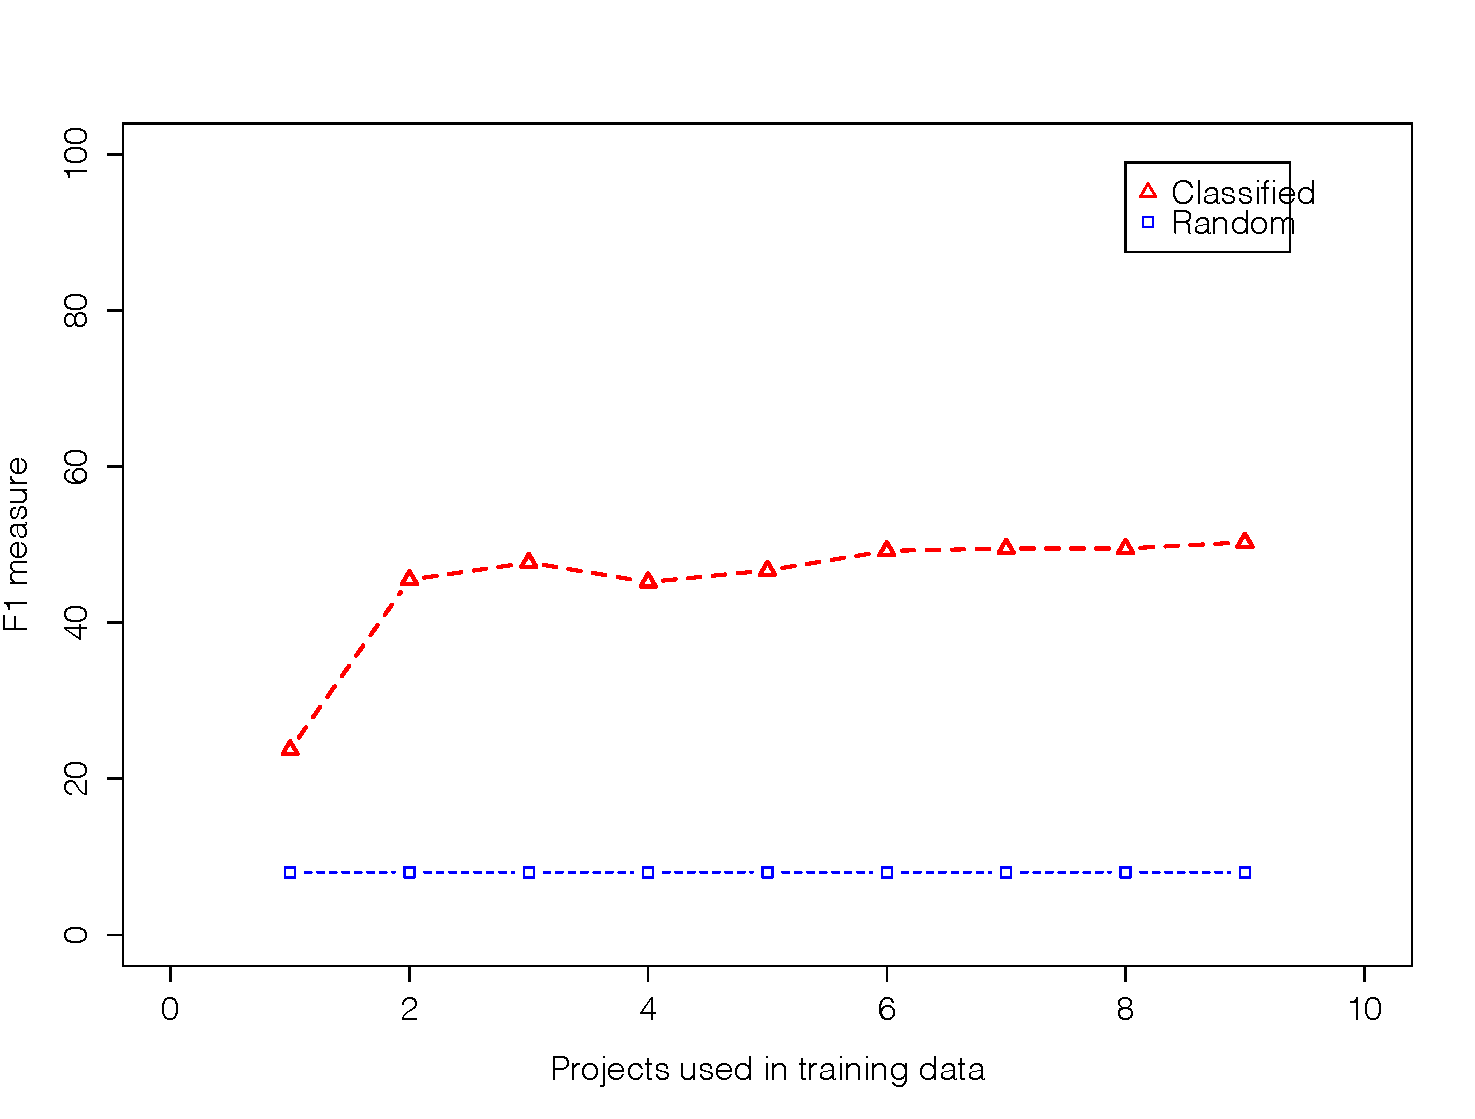
\includegraphics[width=0.48\textwidth]{figures/design_jfreechart.pdf}
  \vspace{-3mm}
  \caption{JFreeChart Design Debt classification}
  \label{fig:design_jfreechart_result}
\end{figure}

\begin{figure}[thb!]
  \centering
  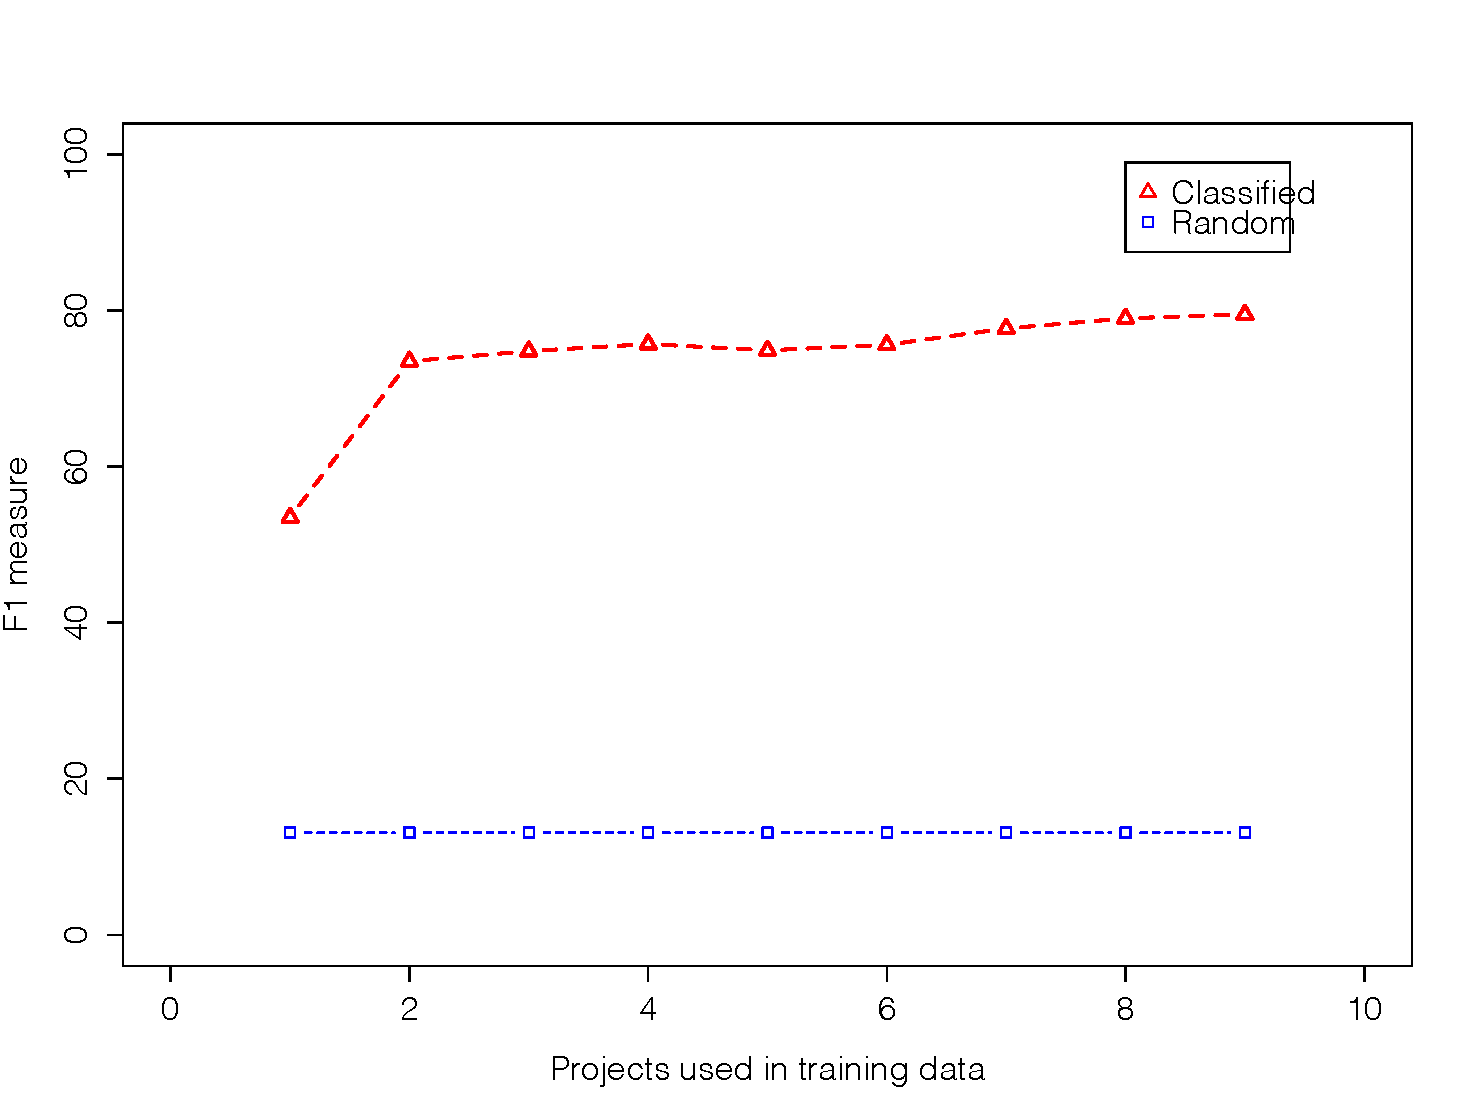
\includegraphics[width=0.48\textwidth]{figures/design_jruby.pdf}
  \vspace{-3mm}
  \caption{JRuby Design Debt classification}
  \label{fig:design_jruby_result}
\end{figure}

Table \ref{tbl:design_iteration_performance} summarizes how much the F1 measure of each iteration represents of the maximum F1 measure in average.  

\begin{table}[!hbt]
    \begin{center}
        \caption{Iteration performance compared with maximum F1 measure for Design Debt}
        \label{tbl:design_iteration_performance}
        \begin{tabular}{l| c c }
        \toprule
        \thead{Iteration\\Number} & \thead{\% of maximum\\F1 measure} & \thead{Average\\comments} \\
        \midrule
         1  &  0.684  & 756 \\  
         2  &  0.805  & 1,106 \\  
         3  &  0.863  & 1,444 \\  
         4  &  0.879  & 1,717 \\  
         5  &  0.857  & 1,919 \\  
         6  &  0.931  & 2,108 \\  
         7  &  0.950  & 2,251 \\  
         8  &  0.958  & 2,353 \\  
         9  &  0.966  & 2,432 \\  
        \bottomrule
        \end{tabular}
    \end{center}    
\end{table}

% While classifying Requirement \SATD comments we find that the first iteration has a goo
% because there is no space for showeing all the figures we present in this table the average f1 measure obtained during each interation for all the projects. The third column of this table shows the average of comments used in each execution to achieve the shown f1 measure. 

\conclusionbox{}